% 2009 年浙江卷理科第 17 题：长方形 ABCD 及 △AFD 沿 AF 折起后的图形。
% 来源 PDF：普通高考/2009/2009浙江理.pdf，SHA-256 8b9a62d8af65c0049a04b2c462e5bc8dc66a464244ca2c2462c6cdfafc5c2d89。
% 原页：第 1 页第 3 栏中部，书页码 565。
% 重绘依据：左图为长方形 ABCD（AB=2、BC=1），E 为 DC 中点（原页标出黑点），
%   F 在 EC 上，AF 为折痕；右图为折起后的情形，A、K、B 共线，DK⊥AB，
%   D 在 K 的正上方，F 为折痕与底面的交点，C 在右下。
%   原页中以虚线表示的 A—F、D—F 在此按原样保留为虚线；D—C 为原页实线，照录。
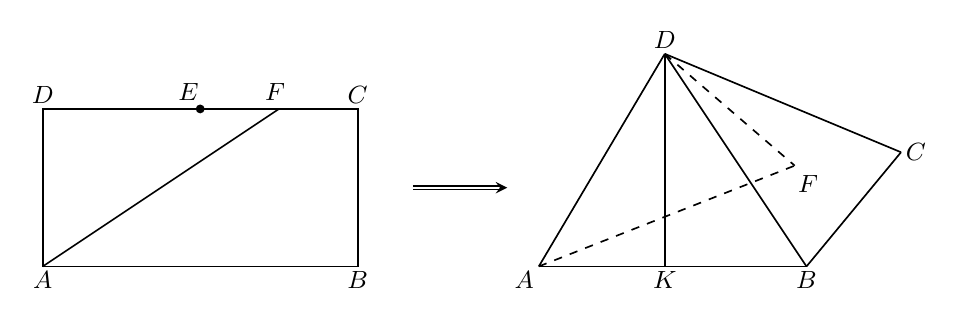
\begin{tikzpicture}[semithick, every node/.style={inner sep=1.5pt, font=\small}]

  % ---------- 折前 ----------
  \draw (0,0) rectangle (4,2);
  \draw (0,0) -- (3,2);
  \fill (2,2) circle (1.6pt);
  \node[above] at (0,2) {$D$};
  \node[above] at (1.85,2.05) {$E$};
  \node[above] at (2.95,2.05) {$F$};
  \node[above] at (4,2) {$C$};
  \node[below] at (0,0) {$A$};
  \node[below] at (4,0) {$B$};

  % ---------- 箭头 ----------
  \draw[double, ->, >=stealth] (4.7,1.0) -- (5.9,1.0) node[midway, above] {};

  % ---------- 折后 ----------
  \coordinate (A) at (6.3,0);
  \coordinate (K) at (7.9,0);
  \coordinate (B) at (9.7,0);
  \coordinate (D) at (7.9,2.7);
  \coordinate (C) at (10.9,1.45);
  \coordinate (F) at (9.55,1.28);
  \draw (A) -- (B);
  \draw (A) -- (D);
  \draw (D) -- (K);
  \draw (D) -- (B);
  \draw (B) -- (C);
  \draw (D) -- (C);
  \draw[dashed] (A) -- (F);
  \draw[dashed] (D) -- (F);
  \node[below left] at (A) {$A$};
  \node[below] at (K) {$K$};
  \node[below] at (B) {$B$};
  \node[above] at (D) {$D$};
  \node[right] at (C) {$C$};
  \node[below] at (9.72,1.22) {$F$};
\end{tikzpicture}
